\documentclass[dvipsnames, usenames]{beamer}

\usetheme{cleancode}
\usepackage[T1]{fontenc}
\usepackage[ansinew]{inputenc}
\usepackage[USenglish]{babel}
\usepackage{amsmath}
\usepackage{mathtools}
\usepackage{stmaryrd}
\usepackage{graphicx}
\usepackage{lmodern}
%\usepackage{tcolorbox}

\usepackage[round, authoryear]{natbib}
\usepackage{subcaption}
\usepackage[export]{adjustbox}

% Graph Picture Packages
\usepackage{tikz}
\usetikzlibrary{positioning}
\usetikzlibrary{calc}

\usepackage{amsthm, amssymb, amsfonts, amsmath, xcolor}
\def\boxitem#1{\setbox0=\vbox{#1}{\centering\makebox[0pt]{%
  \fboxrule=2pt\color{red}\fbox{\hspace{\leftmargini}\color{black}\box0}}\par}}


\usepackage{algorithm,algorithmicx,algpseudocode}
\algnewcommand\algorithmicinput{\textbf{Input:}}
\algnewcommand\INPUT{\item[\algorithmicinput]}
\algnewcommand\algorithmicoutput{\textbf{Output:}}
\algnewcommand\OUTPUT{\item[\algorithmicoutput]}
\algnewcommand\algorithmicidea{\textbf{Idea:}}
\algnewcommand\IDEA{\item[\algorithmicidea]}
\algnewcommand\algorithmicinit{\textbf{Initialize:}}
\algnewcommand\INIT{\item[\algorithmicinit]}

\algnewcommand\algorithmicforeach{\textbf{for each}}
\algdef{S}[FOR]{ForEach}[1]{\algorithmicforeach\ #1\ \algorithmicdo}


\newcommand\Wider[2][3em]{%
\makebox[\linewidth][c]{%
  \begin{minipage}{\dimexpr\textwidth+#1\relax}
  \raggedright#2
  \end{minipage}%
  }%
}

\usepackage{bibentry, bibentry}

% Generates new title page at beginning of each section
\AtBeginSection[]{
  \begin{frame}
  \vfill
  \centering
  \begin{beamercolorbox}[sep=8pt,center,shadow=true,rounded=true]{title}
    \usebeamerfont{title}\insertsectionhead\par%
  \end{beamercolorbox}
  \vfill
  \end{frame}
}
\setbeamertemplate{navigation symbols}{}


\DeclareMathOperator*{\plim}{plim}

\setbeamertemplate{footline}[frame number]
\setbeamertemplate{theorems}[numbered]

\newcommand{\R}{\mathbb{R}}
\newcommand{\N}{\ensuremath{\mathcal{N}}}

\pgfdeclareimage[width=0.7\paperwidth]{mybackground}{../figures/report/datasets}
%
%\setbeamertemplate{title page}{
%
%        \begin{picture}(0,0)
%
%            \put(-30,-100){%
%                \pgfuseimage{mybackground}
%            }
%
%            \put(0,-110.7){%
%                \begin{minipage}[b][45mm][t]{226mm}
%                    \usebeamerfont{title}{\inserttitle\par}
%                    	\usebeamerfont{author}{\insertauthor\par}
%                \end{minipage}
%            }
%
%            \end{picture}
%
%    }

\usepackage{enumitem,amssymb}
\newlist{todolist}{itemize}{2}
\setlist[todolist]{label=$\square$}
\usepackage{pifont}
\newcommand{\cmark}{\ding{51}}%
\newcommand{\xmark}{\ding{55}}%
\newcommand{\done}{\rlap{$\square$}{\raisebox{2pt}{\large\hspace{1pt}\cmark}}%
\hspace{-2.5pt}}
\newcommand{\wontfix}{\rlap{$\square$}{\large\hspace{1pt}\xmark}}


\usepackage[customcolors]{hf-tikz}

\hfsetfillcolor{white}
\hfsetbordercolor{red}
\usepackage{tcolorbox}

\begin{document}

%------------------------------------------------------------------------------%
% Setup TikzStyle

\tikzstyle{block} = [rectangle, draw, 
    text width=5em, text centered, rounded corners, minimum height=1.5em]
    
\tikzstyle{line} = [draw, -latex]

\title{Biologically Plausible Deep Learning: \\ A Critical Review of \citet{guerguiev2017} \thanks{Guerguiev, J., Lillicrap, T. P., \& Richards, B. A. (2017). Towards deep learning with segregated dendrites. ELife, 6, e22901.}}
\subtitle{}

\author{\texorpdfstring{Robert Tjarko Lange\thanks{Code: \url{github.com/RobertTLange/Bio-Plausible-DeepLearning}}
						\newline\url{rtl17@ic.ac.uk}
						\newline\url{www.rob-lange.com}
	}
	{Author}}


\institute{Einstein Center for Neurosciences Berlin}
\date{\today}


%------------------------------------------------------------------------------%

\begin{frame}[noframenumbering]

\titlepage
%\begin{picture}(0,0)
%\put(+25,+0){\pgfuseimage{mybackground}}
%\end{picture}
\end{frame}

%------------------------------------------------------------------------------%
\begin{frame}{Motivation - Backpropagation}

\begin{itemize}
	\item[$\rightarrow$] MLP: Composition of layers $\{h_l\}_{l=1}^L$, $h_0 = x$, $\theta_l =\{W_l, b_l\}$ and "Learn" synaptic weights, $\Theta = \{\theta_l\}_{l=1}^L$ iteratively. 
	\vspace{-0.5cm}

\begin{align*}
h_l \coloneqq f(h_{l-1}; \theta_l) &= \sigma_l (W_l h_{l-1} + b_l)\\
\min_\theta \mathcal{L}(h_L|\Theta) &= - \sum_y q(y|x) \log p(y|h_L; \Theta)
\end{align*}
	\pause
	\item[$\rightarrow$] Backpropagation:
	\vspace{-0.5cm}

\begin{align*}
	\frac{\partial \mathcal{L}}{\partial \theta_l} &= \left(\frac{dh_{l}}{d \theta_{l}}\right)^T \frac{\partial \mathcal{L}}{\partial h_{l}} = \left(\frac{dh_{l}}{d \theta_{l}}\right)^T \left(\frac{dh_{l+1}}{d h_{l}}\right)^T \frac{\partial \mathcal{L}}{\partial h_{l+1}} \\ 
	&=  \left(\frac{dh_{l}}{d \theta_{l}}\right)^T \underbrace{\left(W_{l+1} diag\left(\sigma_{l+1}'(W_{l+1}h_l +b_{l+1})\right)\right)^T}_{\coloneqq \delta_{l+1}} \frac{\partial \mathcal{L}}{\partial h_{l+1}} \\
	&= \left(\frac{dh_{l}}{d \theta_{l}}\right)^T \delta_{l+1} \delta_{l+2}\frac{\partial \mathcal{L}}{\partial h_{l+2}} = \dots 
\end{align*}
\end{itemize}
\end{frame}

%------------------------------------------------------------------------------%
\begin{frame}{Motivation - Problems with Backpropagation}
\vspace{-0.5cm}

\begin{equation*}
	\frac{\partial \mathcal{L}}{\partial \theta_l} 
	=  \left(\frac{dh_{l}}{d \theta_{l}}\right)^T \left(\prod_{i=l+1}^L \delta_i\right) \frac{\partial \mathcal{L}}{\partial h_{L}}
\end{equation*}

\begin{todolist}
\item[\wontfix] \textbf{Weight Transport Problem} \pause
\item[\wontfix] \textbf{Global signed error signal} \pause
\item[\wontfix] \textbf{Computationally Expensive Matrix Transposition} \pause
\item Alternatives:
\begin{itemize}
	\item[$\circ$] Feedback Alignment \citep{lillicrap2016}
	\item[$\circ$] Target Propagation \citep{lee2015}
\end{itemize}
\pause
\item Problems with Alternatives:
\begin{itemize}
	\item[$\circ$] Need form of info transmission to determine local errors 
	\item[$\circ$] Not possible in single compartment neurons without feedback pathway
\end{itemize}
\end{todolist}
\end{frame}


%------------------------------------------------------------------------------%
\begin{frame}{Motivation - Electrical Segregation of $\downarrow$ and $\uparrow$ Info}

\begin{tabular}{cl}  
    \begin{tabular}{c}
           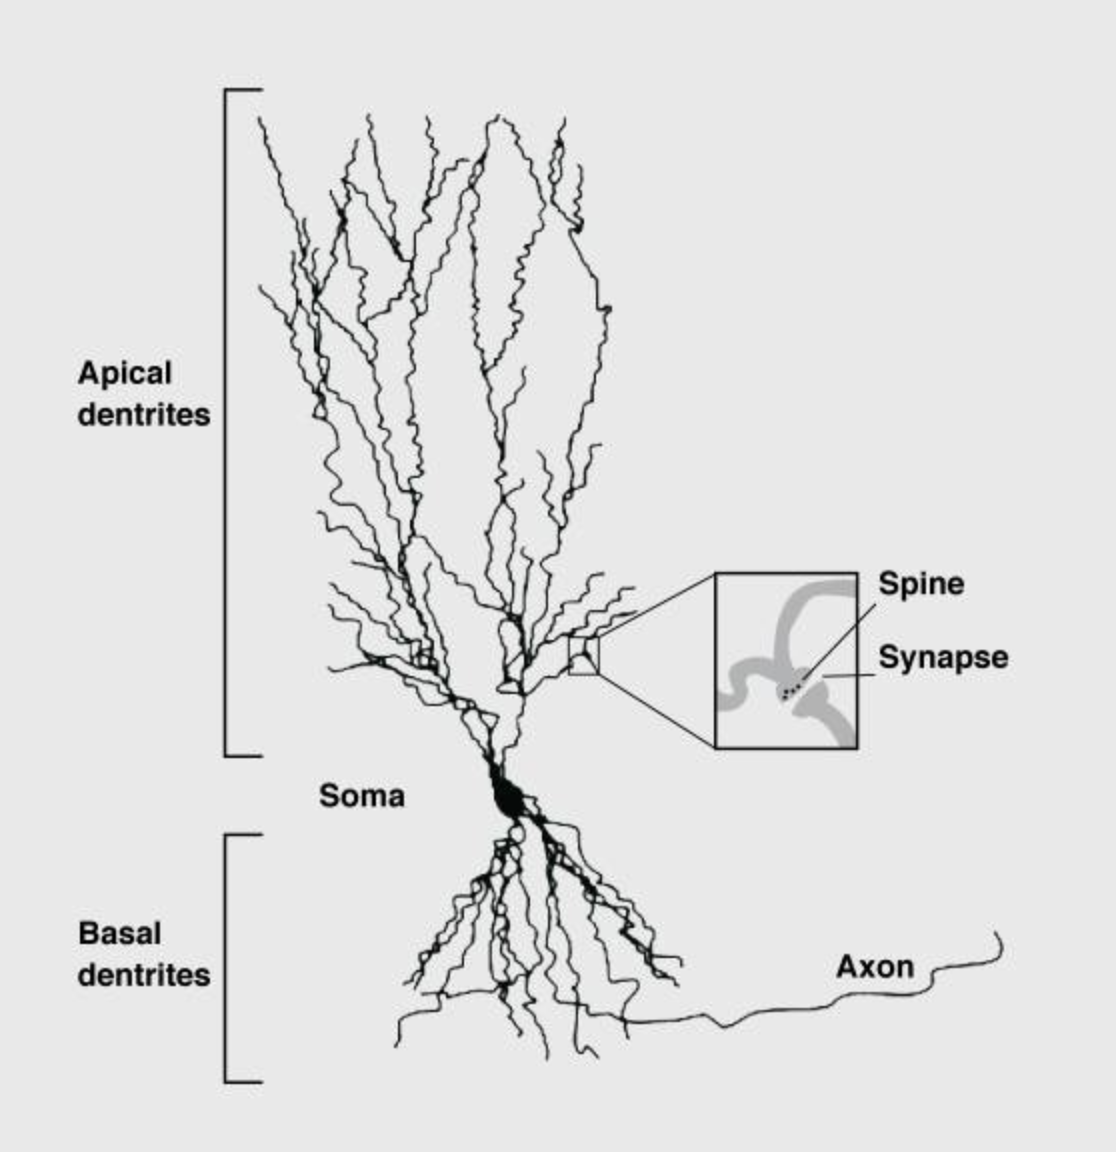
\includegraphics[height=5cm, width=5cm]{../figures/report/pyramidal_ca3}
           \end{tabular}
           & \begin{tabular}{l}
             \parbox{0.45\linewidth}{%  change the parbox width as appropiate
             \begin{itemize}
             	\item[$\rightarrow$] \citet{kording2001}: Local error computation via electrical segregation
             	\item[$\rightarrow$] Multi-compartmental segregation avoids need for feedback pathway
             	\item[$\rightarrow$] Apical dendrites ($\Downarrow$)
				\item[$\rightarrow$] Basal dendrites ($\Uparrow$)
             \end{itemize} 
    }
         \end{tabular}  \\
\end{tabular}
\pause
\begin{itemize}
		\item[$\rightarrow$] \textbf{Plateau Potentials}:
	\begin{itemize}
		\item[$\circ$] Apical $\Rightarrow$ soma via voltage-gate $Ca^{2+}$ channels
		\item[$\circ$] Prolonged upswing in MP due to events in apical shaft
		\item[$\Rightarrow$] Can guide plasticity in pyramidal neurons
	\end{itemize}
\end{itemize}
\end{frame}

%------------------------------------------------------------------------------%
\begin{frame}{\citet{guerguiev2017} - Neuron and Network Model}

\begin{itemize}
	\item[$\to$] 3 Compartment Hidden Layer: $\mathbf{V}^{0a}(t), \mathbf{V}^{0b}(t), \mathbf{V}^{0}(t) \in \R^m$
\end{itemize}	
	\begin{align*}
		\tau \frac{dV_i^0(t)}{dt} &= -V_i^0(t) + \frac{g_b}{g_l}\left(V_i^{0b}(t) - V_i^0(t)\right) +\frac{g_a}{g_l}\left(V_i^{0a}(t) - V_i^0(t)\right)\\
		V_i^{0b} &= \sum_{j=1}^l W_{ij}^0 s_j^{input}(t) + b_i^0 \ \ \text{and} \ \ V_i^{0a} = \sum_{j=1}^n Y_{ij} s^1_j(t)
	\end{align*}
\begin{itemize}
\pause
	\item[$\to$] 2 Compartment Output Layer: $\mathbf{V}^{1b}(t), \mathbf{V}^{1}(t) \in \R^n$
\end{itemize}
\begin{align*}
		\tau \frac{dV_i^1(t)}{dt} &= -V_i^1(t) + \frac{g_d}{g_l}\left(V_i^{1b}(t) - V_i^1(t) \right) + I_i(t)\\
		V_i^{1b} &= \sum_{j=1}^l W_{ij}^1 s_j^{0}(t) + b_i^1
\end{align*}
\begin{itemize}
	\item[$\to$] $s_j^{input}(t) = \sum_k \kappa(t-t_{jk}^{input})$ with $\kappa$ response kernel
	\end{itemize}
\end{frame}

%------------------------------------------------------------------------------%
\begin{frame}{\citet{guerguiev2017} - Credit Assignment Signals}

\begin{itemize}
	\item[$\to$] \textbf{Forward} ($t_0 + \Delta t_s \to t_1$): $I_i(t) = 0, \ \forall i=1,\dots, n$
	\begin{itemize}
		\item[$\circ$] At $t_1$: $\alpha_i^f = \sigma\left(\frac{1}{\Delta t_1} \int_{t_1 - \Delta t_1}^{t_1} V_i^{0a}(t)dt\right)$
	\end{itemize}
	\item[$\to$] \textbf{Target} ($t_1 + \Delta t_s \to t_2$): $I_k(t) = \phi_{max}$ for $y_{sample} = k$
	\begin{itemize}
		\item[$\circ$] At $t_2$: $\alpha_i^t = \sigma\left(\frac{1}{\Delta t_2} \int_{t_2 - \Delta t_2}^{t_2} V_i^{0a}(t)dt\right)$
	\end{itemize}
\end{itemize}
\pause
\begin{figure}
	\centering
	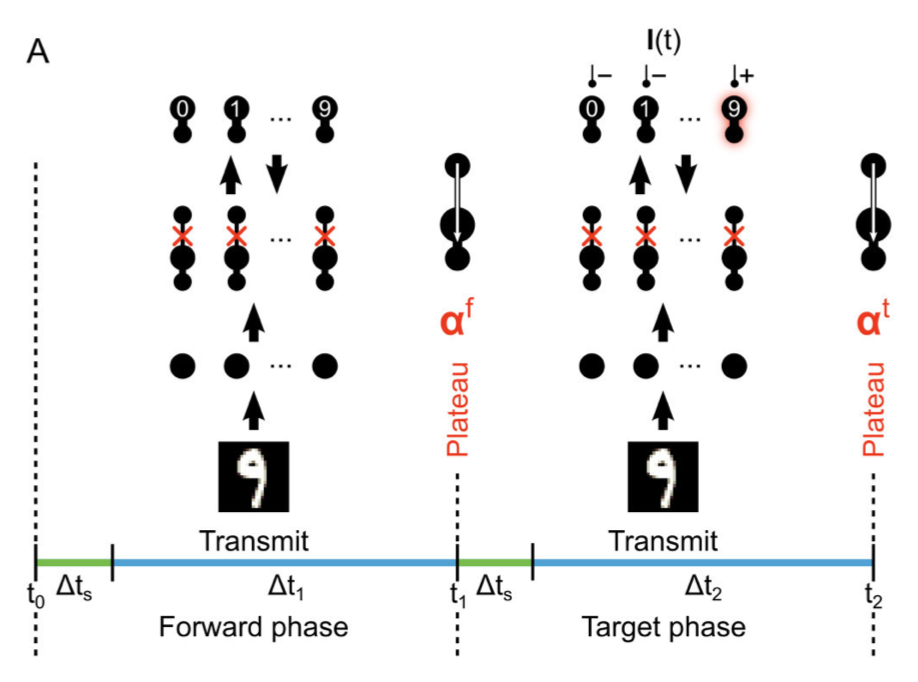
\includegraphics[scale=0.45]{../figures/report/phases}
\end{figure}
         

\end{frame}

%------------------------------------------------------------------------------%
\begin{frame}{\citet{guerguiev2017} - Learning}

\begin{itemize}
	\item[$\to$] How is learning defined in such a model?
	\begin{tcolorbox}

	Forward phase dynamics $\Leftrightarrow$ Target phase dynamics  
	\end{tcolorbox}
	\pause
	\item[$\Rightarrow$] Somatic compartments generate Poisson process spikes:
	\begin{itemize}
		\item[$\circ$] Rates-of-fire: $\phi^l_i(t) = \phi_{max} \sigma(V_i^l(t))$
	\end{itemize}
	\pause
	\item[$\Rightarrow$] Output Layer:
	\begin{itemize}
		\item[$\circ$] Target firing rates: $\phi_i^{1\star} = \frac{1}{\Delta t_2} \int_{t_1 + \Delta t_s}^{t_2} \phi_i^1(t)dt$
		\item[$\circ$] Loss function: $L^1 = ||\phi_i^{1\star} - \bar{\phi}_i^{1f}||_2^2 = ||\frac{1}{\Delta t_2} \int_{t_1 + \Delta t_s}^{t_2} \phi_i^1(t)dt - \frac{1}{\Delta t_1} \int_{t_0 + \Delta t_s}^{t_1} \phi_i^1(t)dt||_2^2$
	\end{itemize}
	\vspace{0.5cm}
	\pause
	\item[$\Rightarrow$] Hidden Layer:
	\begin{itemize}
		\item[$\circ$] Target firing rates: $\phi_i^{0\star} = \bar{\phi}_i^{0f} + \alpha_i^t - \alpha_i^f$
		\item[$\circ$] Loss function: $L^0 = ||\phi_i^{0\star} - \bar{\phi}_i^{0f}||_2^2 = ||\alpha^t - \alpha^f||_2^2$
	\end{itemize}
	\vspace{0.5cm}
	\pause
	\item[$\Rightarrow$] Local error minimization via SGD
\end{itemize}
\end{frame}

%------------------------------------------------------------------------------%

\begin{frame}{Experiments - Learning Dynamics: Performance}
	\begin{figure}
		\centering
		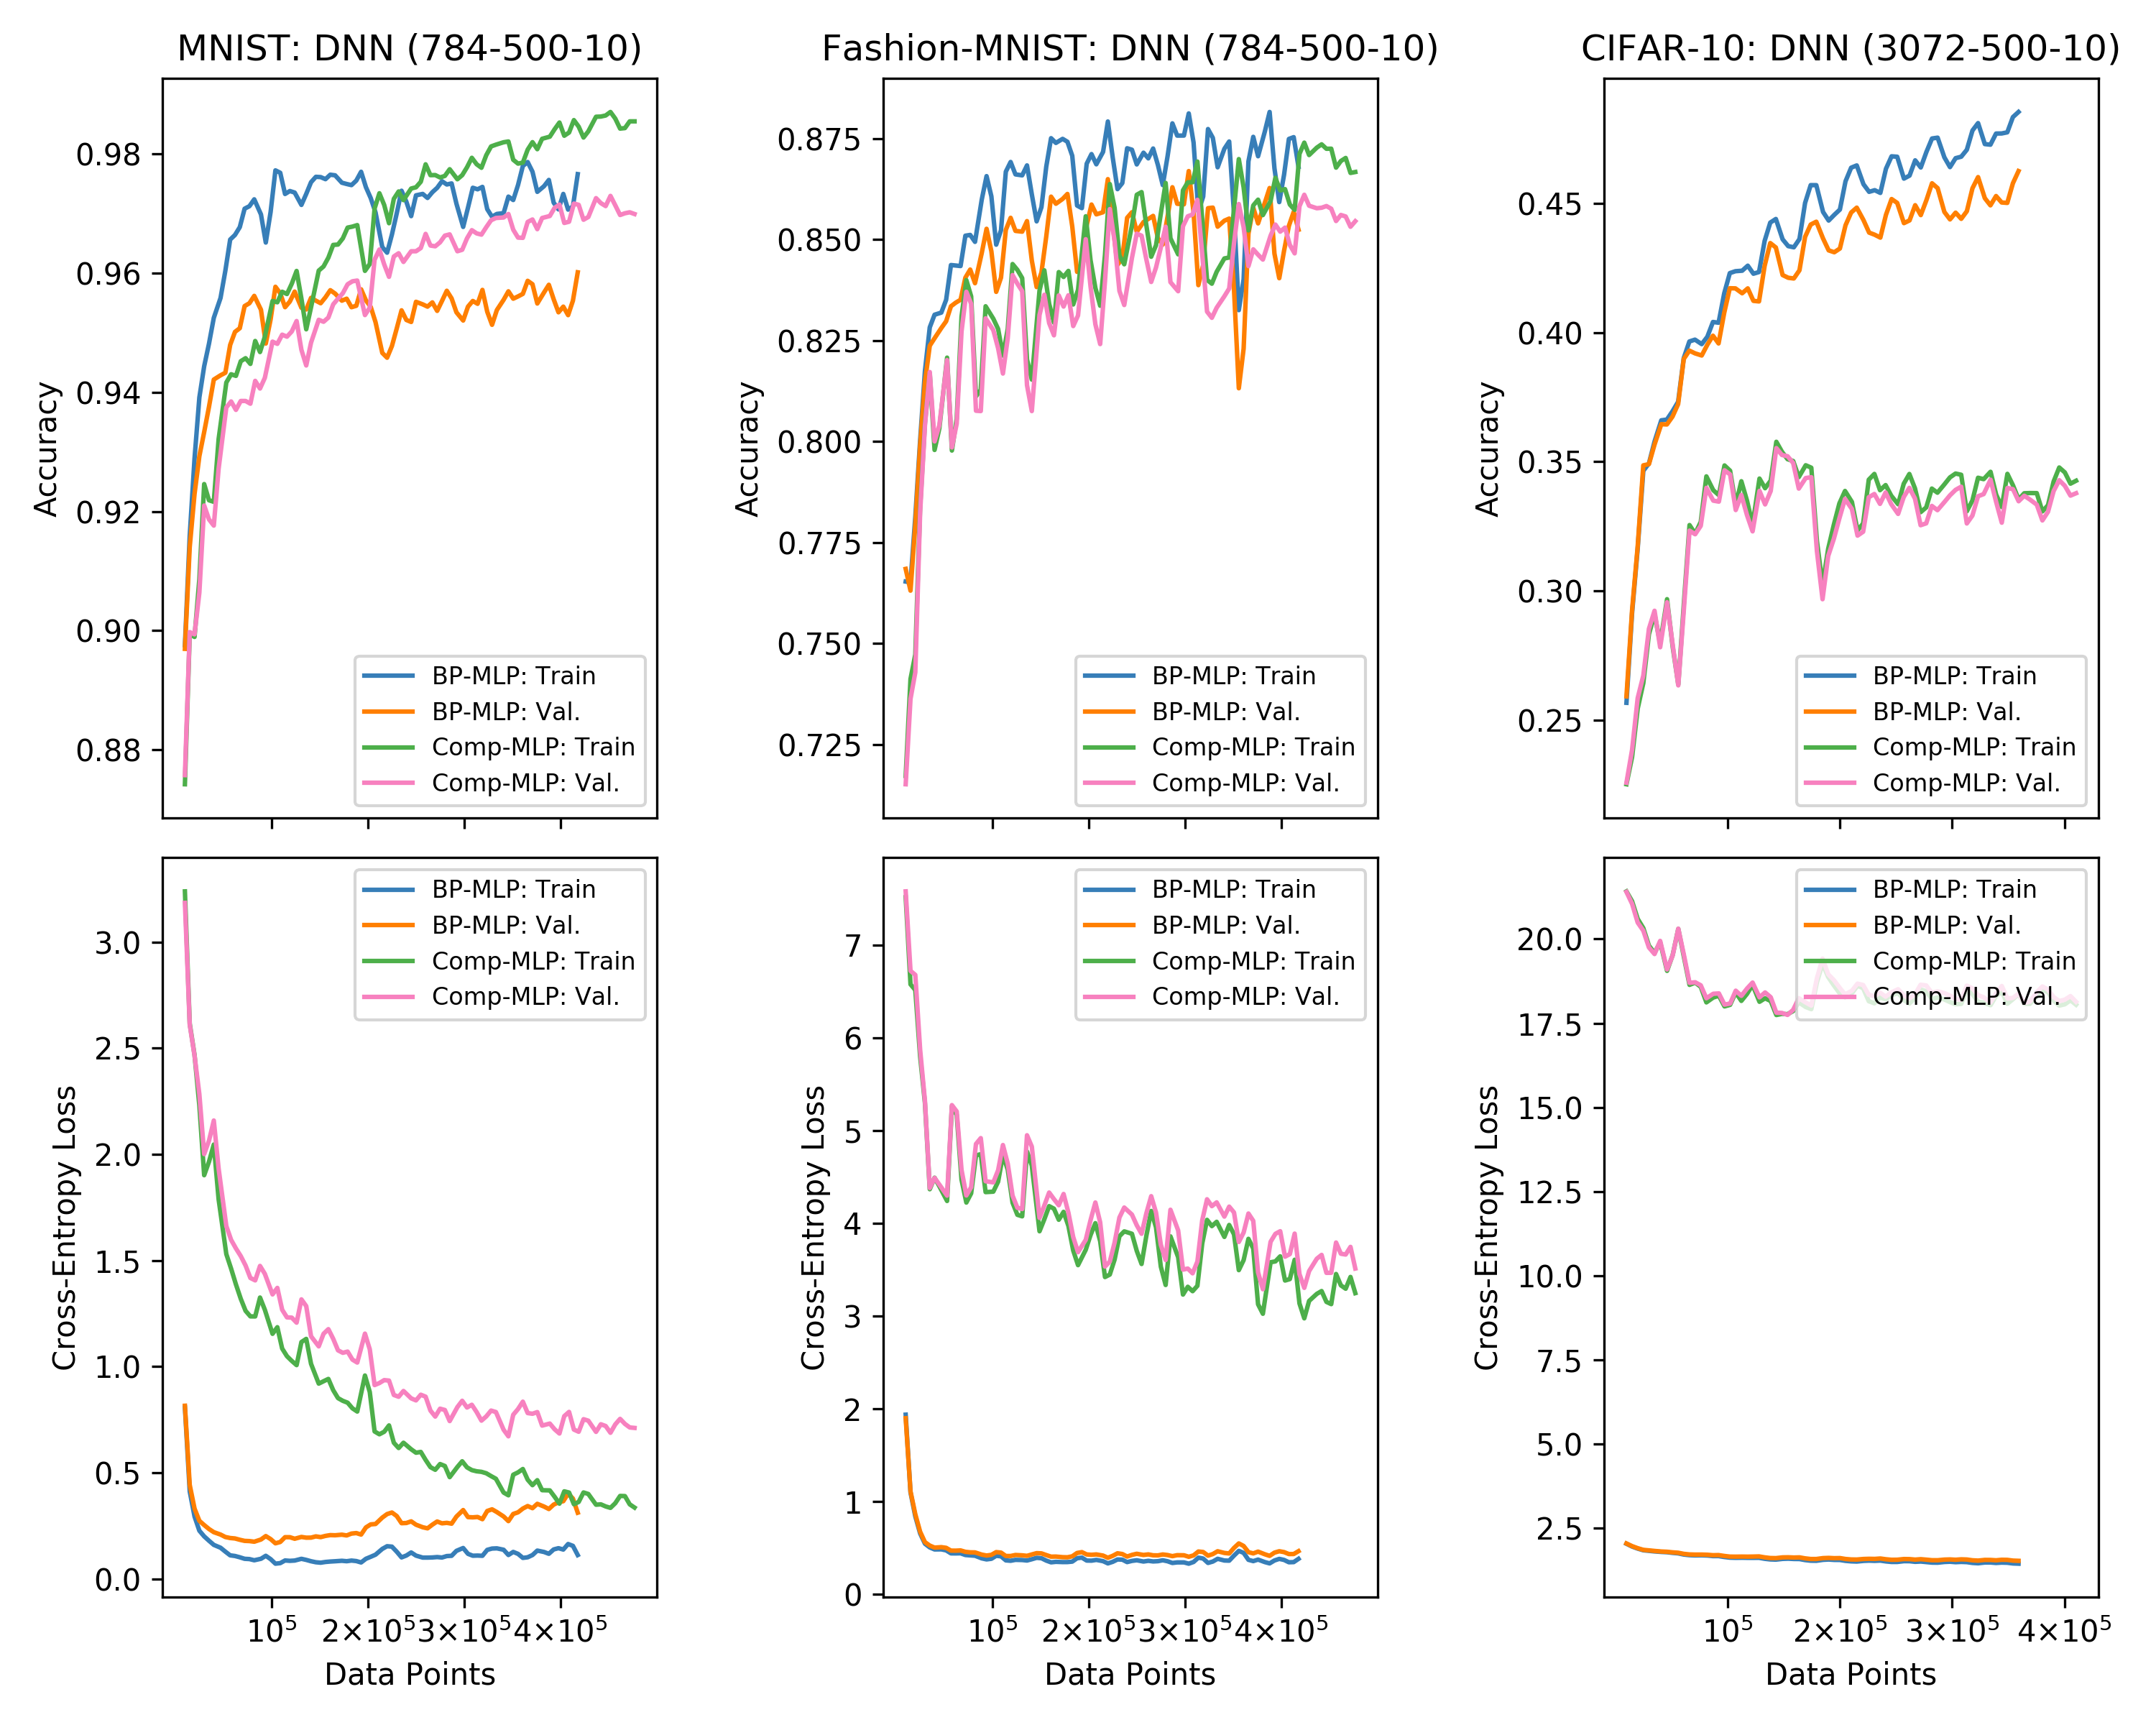
\includegraphics[width=\textwidth]{../figures/learning}
	\end{figure}
\end{frame}

%------------------------------------------------------------------------------%

\begin{frame}{Experiments - Learning Dynamics: Dynamics}
	\begin{figure}
		\centering
		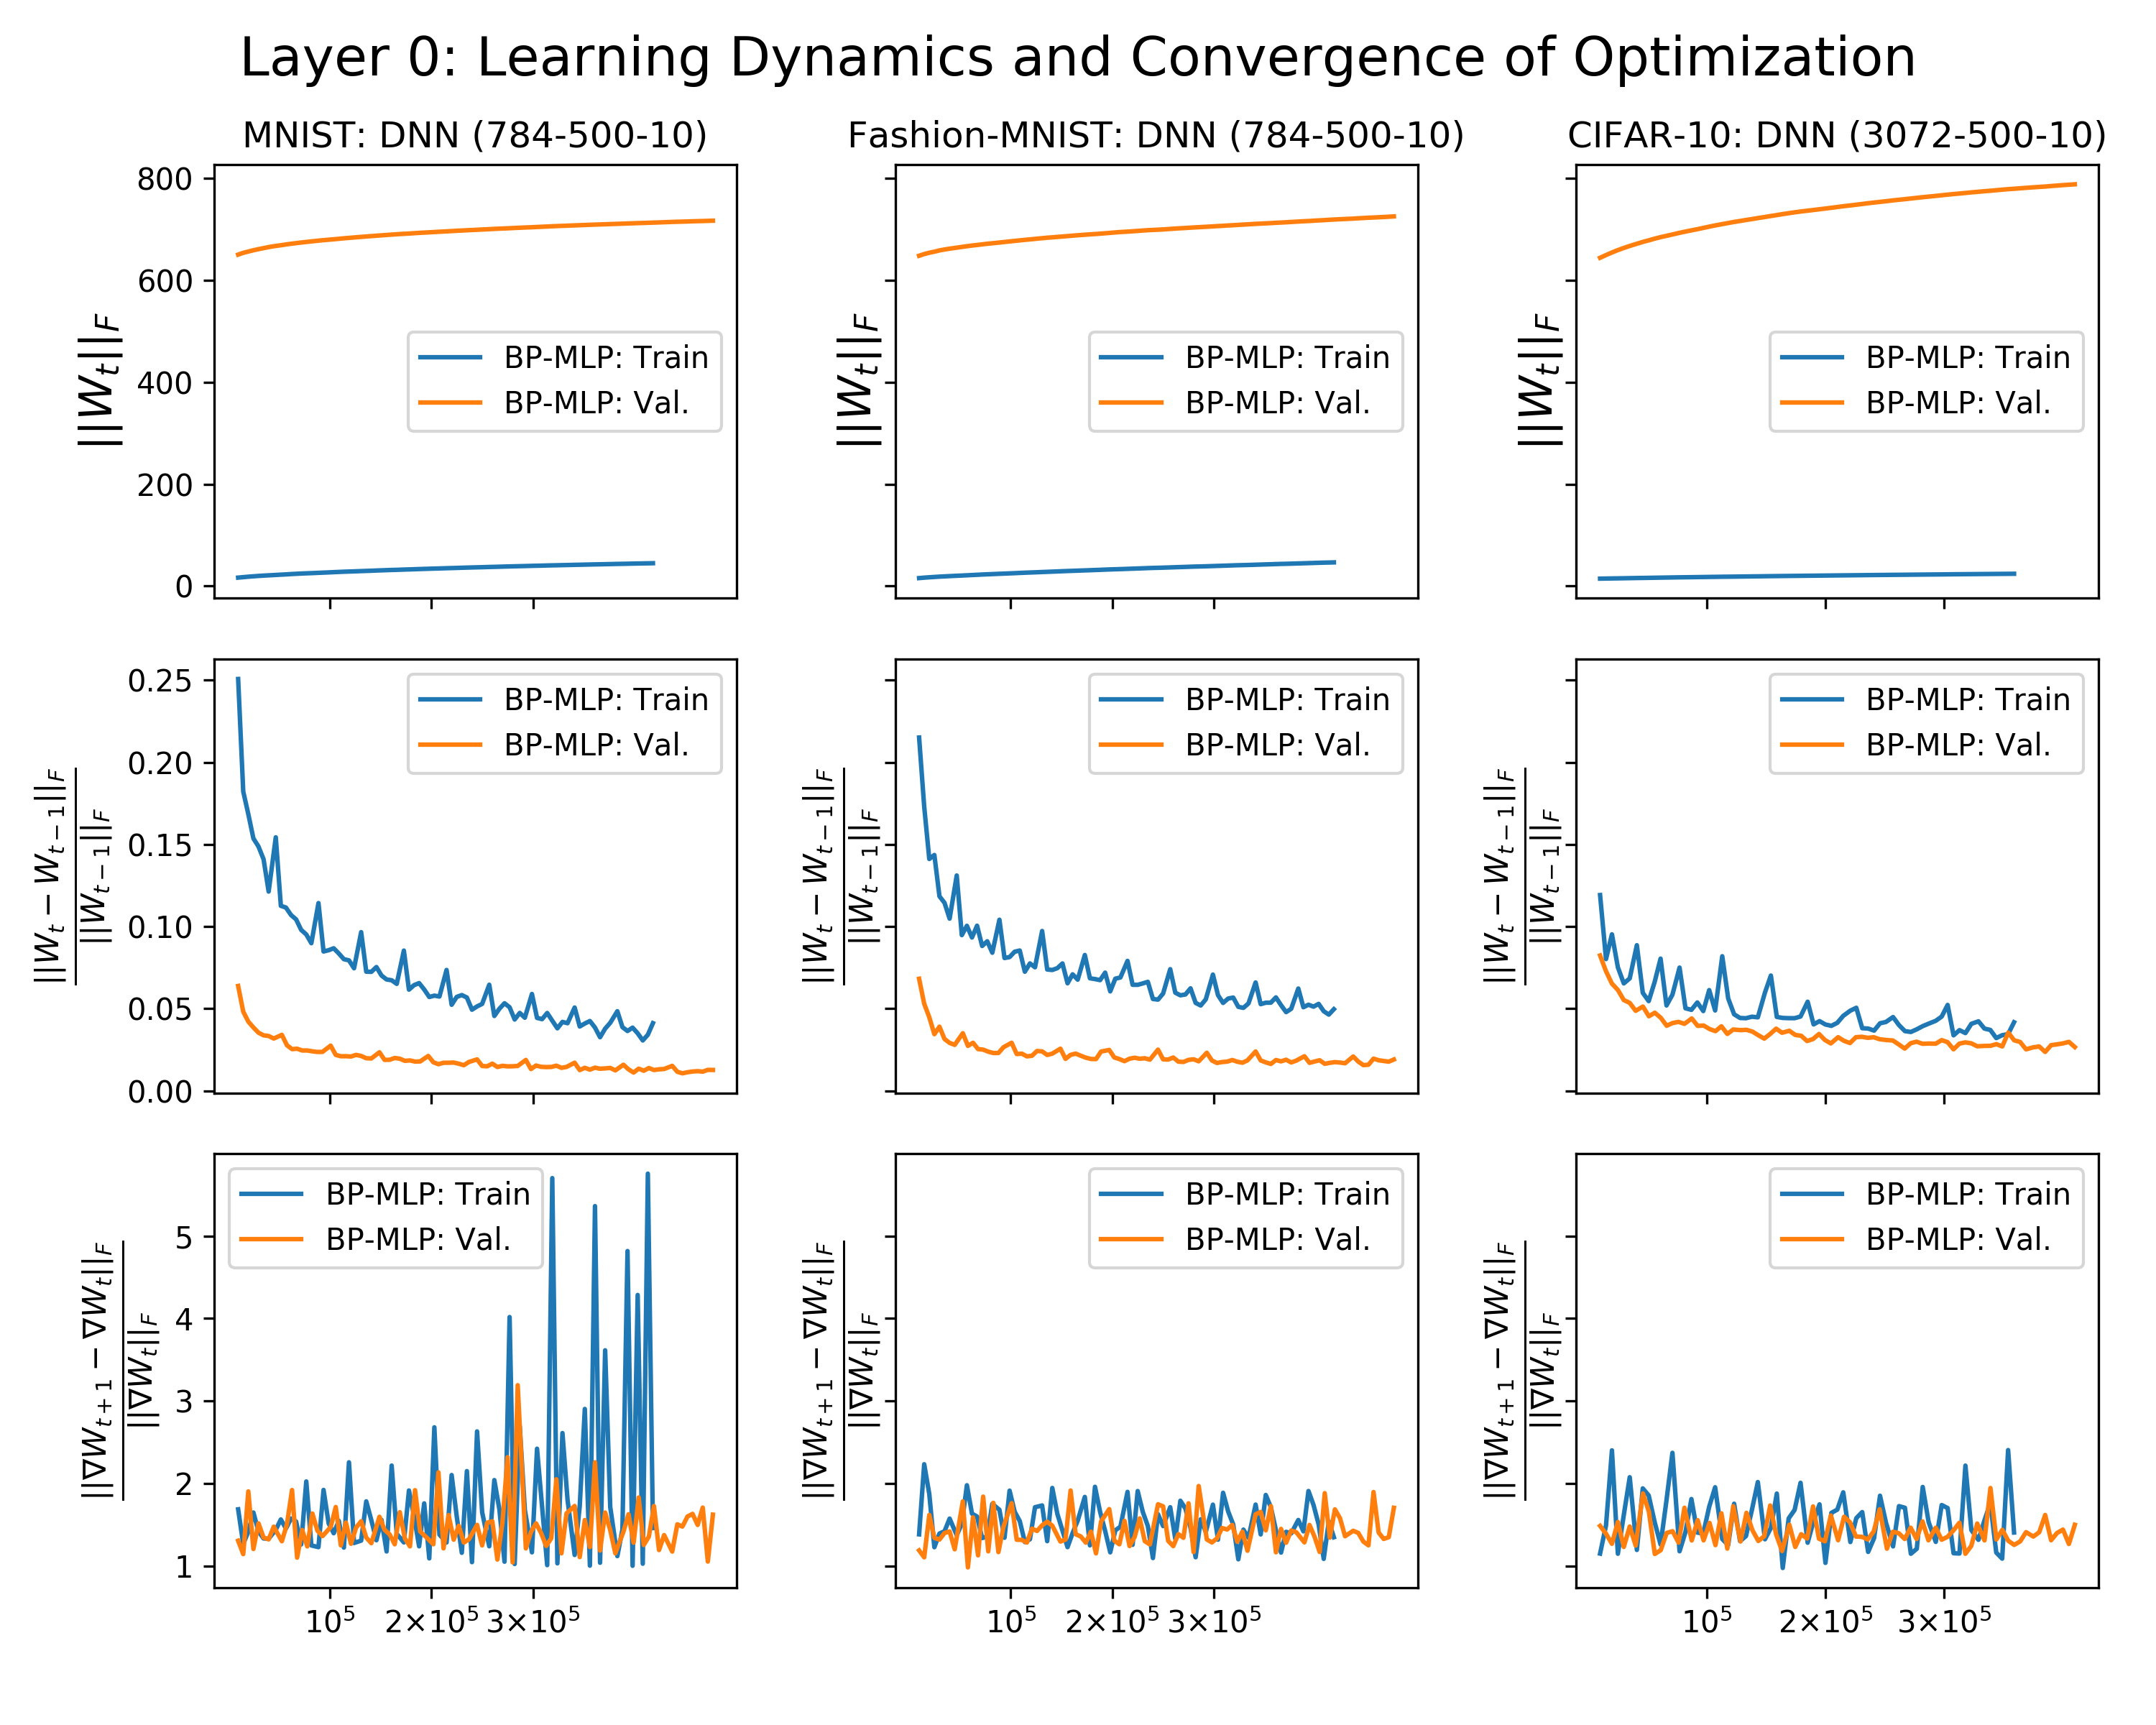
\includegraphics[width=\textwidth]{../figures/dynamics_l0}
	\end{figure}
\end{frame}

%------------------------------------------------------------------------------%

\begin{frame}{Experiments - Learning Dynamics: Robustness}
	\begin{figure}
		\centering
		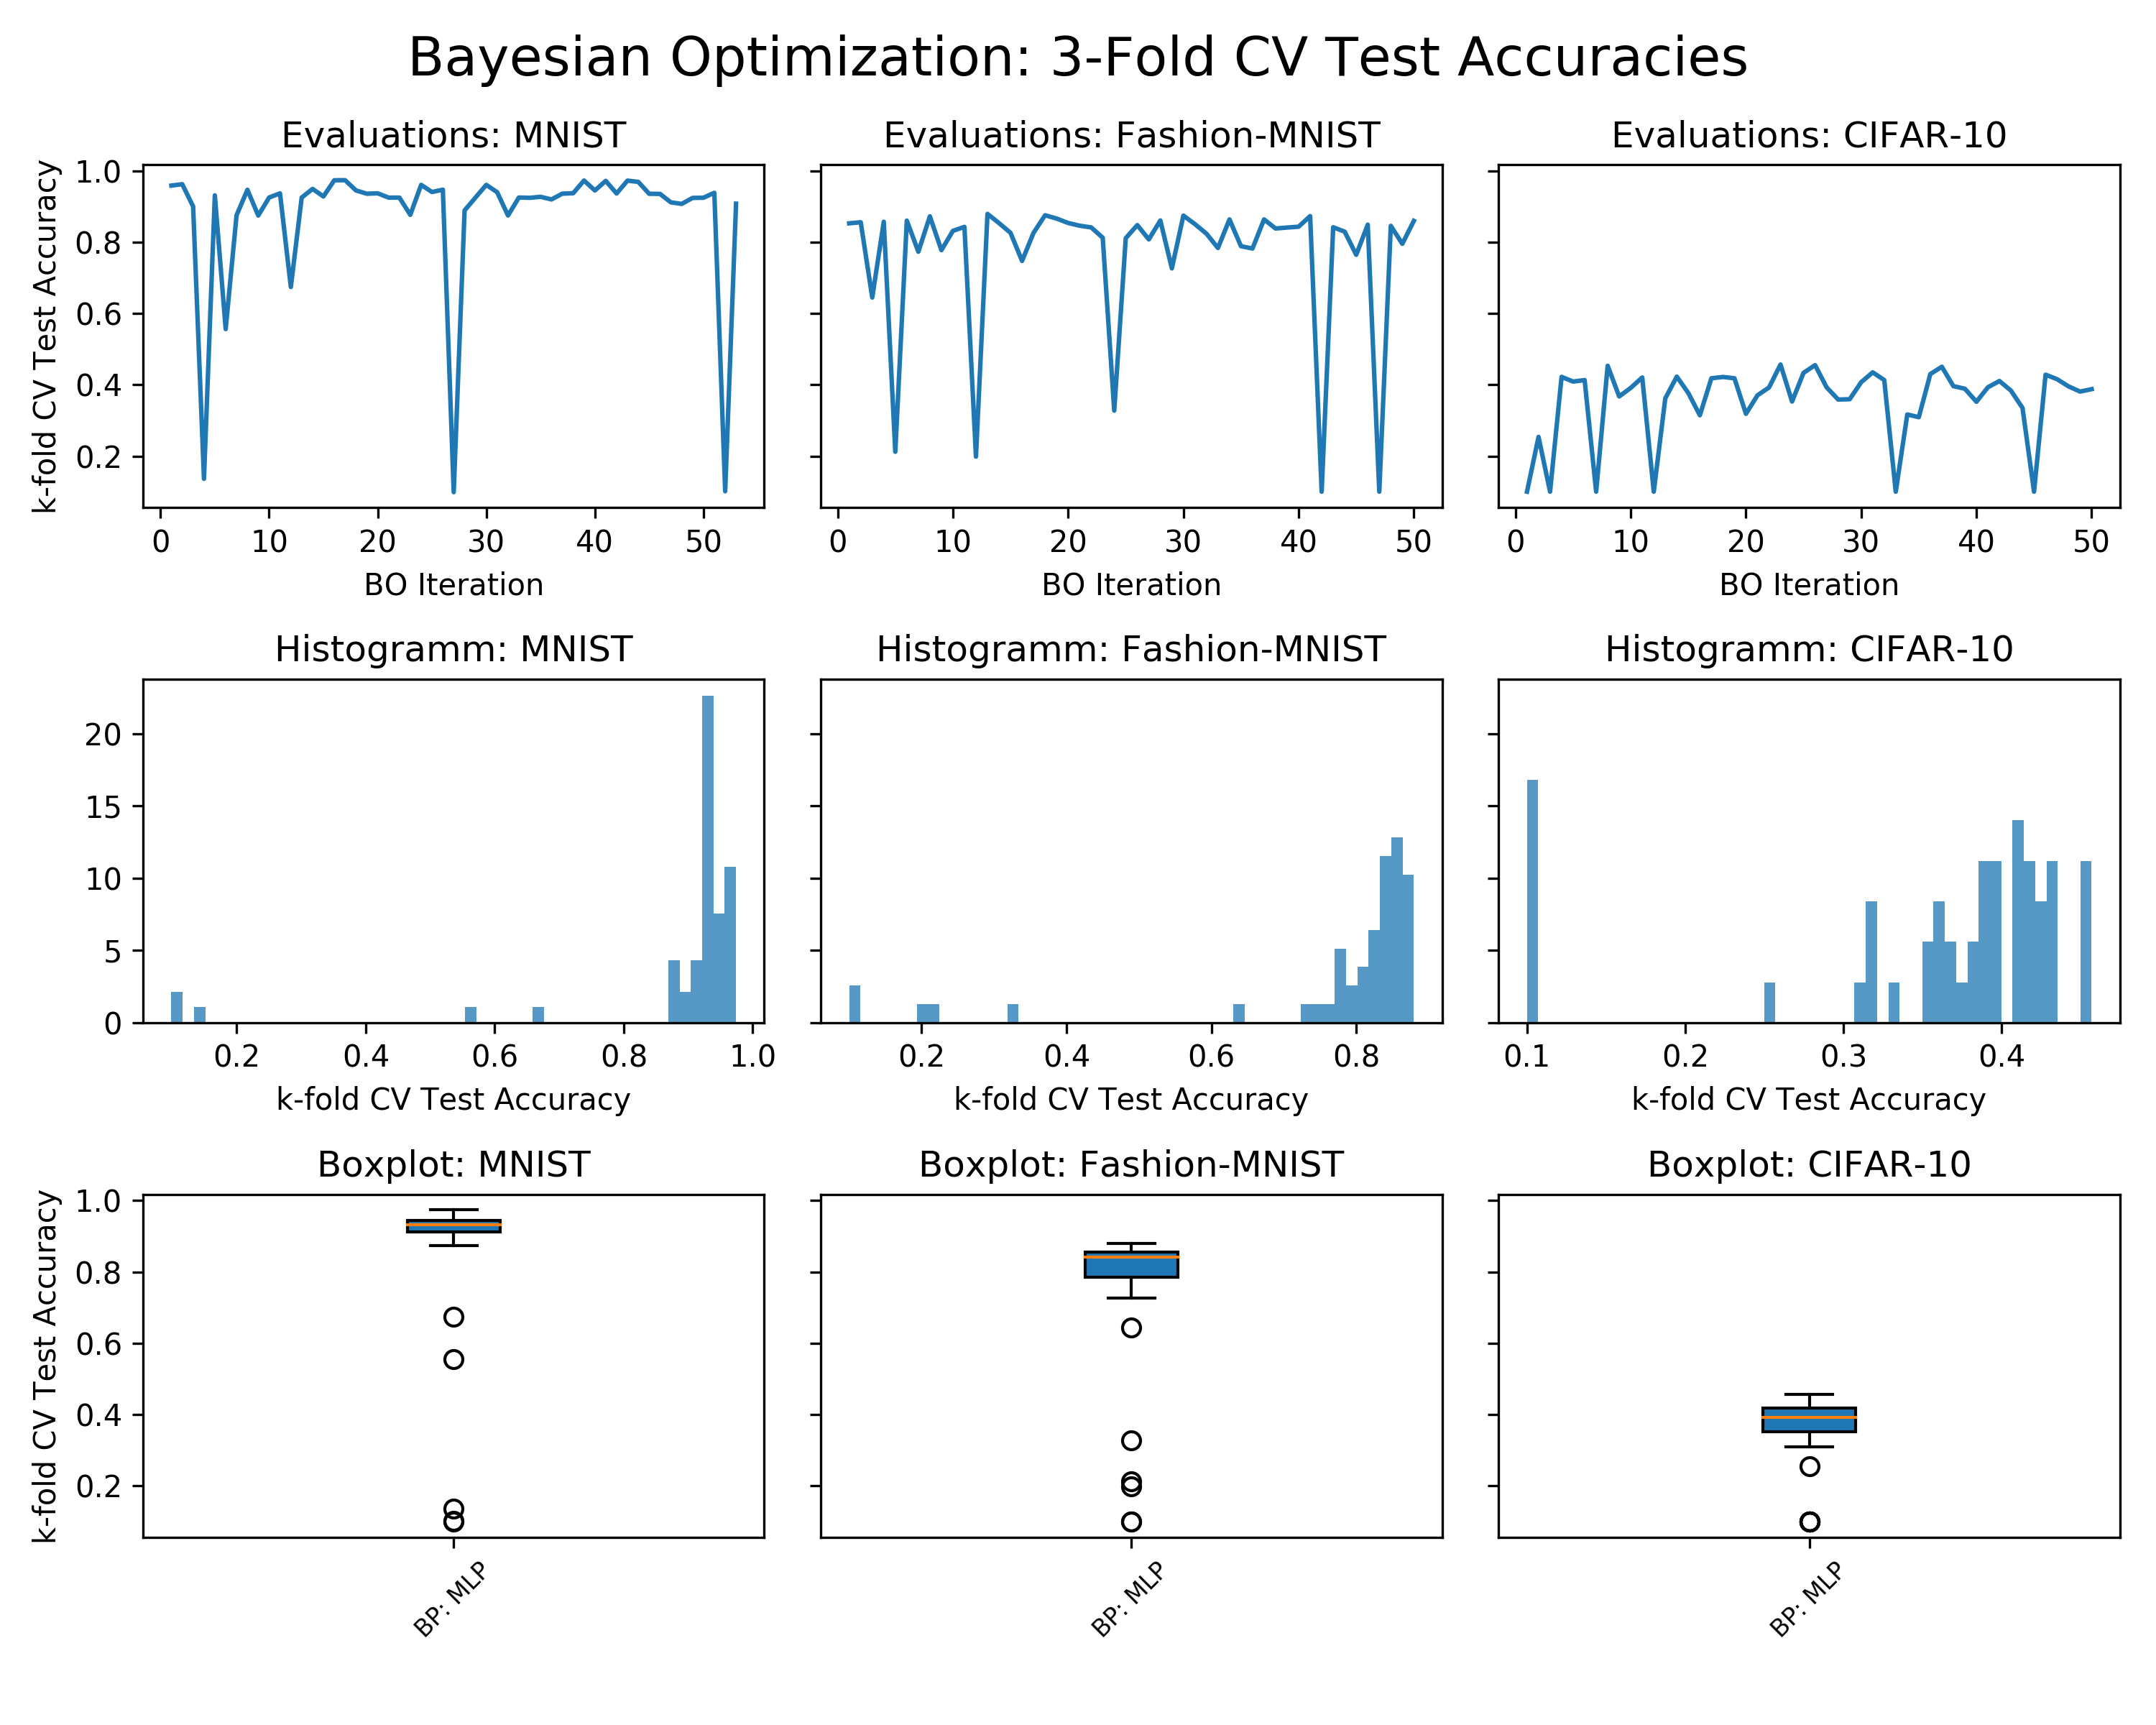
\includegraphics[width=\textwidth]{../figures/bayes_opt_comparison}
	\end{figure}
\end{frame}

%------------------------------------------------------------------------------%
\begin{frame}{\citet{guerguiev2017} - Accomplishments/Problems}

\begin{todolist}
	\item[\done] Segregated compartments generate local targets that act as credit assignment signals in a physiologically plausible manner
	\item[\done] Signal can be used to exploit depth in near-continuous time
	\item[\wontfix] \textbf{Computational} Problems
	\begin{itemize}
		\item[$\rightarrow$] Huge hyperparameter space $\to$ most likely not robust!
	\end{itemize}
	\item[\wontfix] \textbf{Physiological} Problems
	\begin{itemize}
	\item[$\rightarrow$] How is the teaching signal internally generated?
	\item[$\rightarrow$] 2 global phases? - Length sampled from inverse Gaussian
	\item[$\rightarrow$] Stoch. gen. of plateau potentials - apical calcium spikes
	\end{itemize}
	\item[$\Rightarrow$] \citet{sacramento2018}: Neocortical micro-circuits and inhibitory interneurons might act synchronizing.
\end{todolist}
\end{frame}


%------------------------------------------------------------------------------%
\begin{frame}{Literature Review}
\vspace{-0.5cm}

\begin{figure}[H]
	\centering
	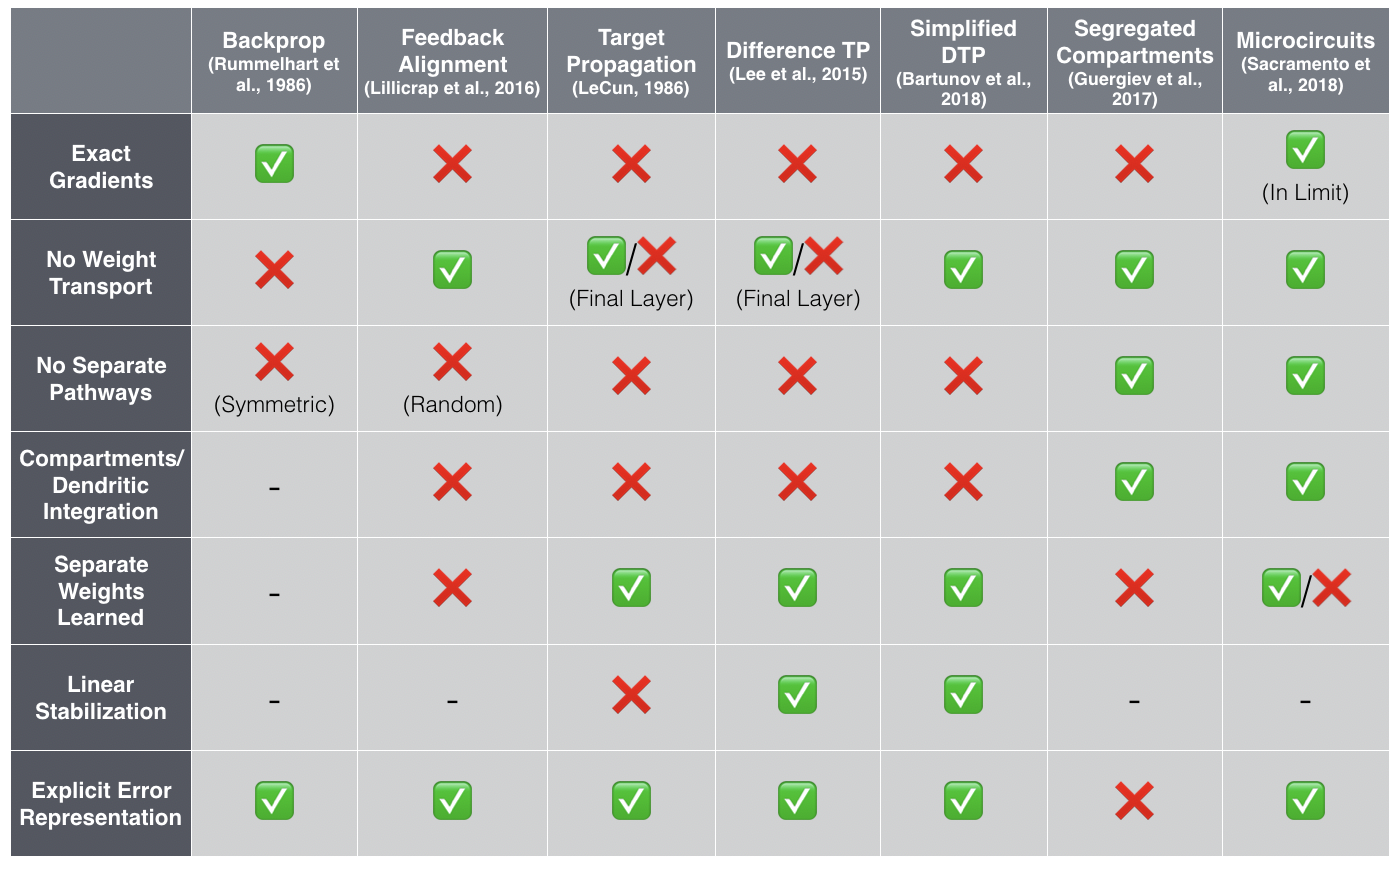
\includegraphics[width=\textwidth]{../figures/report/lit_rev}
\end{figure}

\end{frame}

%------------------------------------------------------------------------------%

\begin{frame}{What do I want to analyze? What's next?}
\vspace{-0.5cm}

\begin{itemize}\footnotesize
  \item Literature Review
  \begin{todolist}
  \item[\done] Feedback Alignment \citep{lillicrap2016}
  \item[\done] Target Propagation \citep{lee2015, bartunov2018},
  \item[\done] Segregated Compartments \citep{guerguiev2017, sacramento2018}
  \end{todolist}
  \item Implement different models/learning rules
  \begin{todolist}
  \item[\done] Standard Backprop MLP, CNN in PyTorch
  \item[\done] Segregated Compartment MLP in Numpy
  \item $k$-fold CV pipeline for SC MLP
  \end{todolist}
  \item Analyze learning dynamics
  \begin{todolist}
  \item $||W_t||_F$ - Overfitting? $||\Delta W_t||_F$ - Convergence? $||\Delta \nabla W_t||_F$ - Local optima? Feedback alignment - Inverse Jacobian
  \item Different SGD variants: Momentum, Adam, RMSprop
  \end{todolist}
  \item Analyze Hyperparameter/Dataset Robustness
  \begin{todolist}
  	\item[\done] Different datasets (MNIST, Fashion, CIFAR-10)
    \item[\done] Bayesian Optimization for Hyperparam. Search Backprop
    \item Bayesian Optimization for Hyperparam. Search SC
  \end{todolist}
\end{itemize}

\end{frame}



%------------------------------------------------------------------------------%

\begin{frame}[allowframebreaks, noframenumbering]{References}
   \begin{tiny}
   \setbeamertemplate{bibliography item}[text]
   \bibliographystyle{authordate1}
   \bibliography{main.bib}
   \end{tiny}
\end{frame}


%------------------------------------------------------------------------------%



\end{document} 